\documentclass{llncs}
%
\usepackage{amsfonts}
\usepackage{amstext}
\usepackage{amsmath}
\usepackage{enumitem}
\usepackage{multirow}
\usepackage{graphicx}
\usepackage[center]{subfigure}
\usepackage{amssymb}
\usepackage{graphicx,amsmath} % Add all your packages here
\usepackage{subfigure}
\usepackage{algorithm}
\usepackage{algorithmic}
\renewcommand{\algorithmicrequire}{ \textbf{Input:}}
\renewcommand{\algorithmicensure}{ \textbf{Output:}}
\usepackage{url}
\usepackage{cite}
\usepackage{color}
%
\begin{document}
	
\title{Title Goes Hear}
\author{Anynimous}
\institute{School of Computer Science and Engineering, Beihang University, Beijing, China\\
%	\email{\{moyuanhuang, w.rong, jiangnan, xiongz\}@buaa.edu.cn}\\
%	\and Department of Computer Science, University of Victoria, Victoria, Canada\\
%	\email{tom.arjannikov@gmail.com}
}
\maketitle

\begin{abstract}
Abstract
\keywords{Keywords1, Keywords2, Keywords3}
\end{abstract}

%For example, it can help music applications like last.fm and NetEase cloud Music to properly recommend music based on the moods of the music pieces.

\section{Introduction}

%Music is important and influential in everyone's life and one of the essential challenges is to conduct music's emotion classification \cite{DBLP:conf/mm/YangLC06}, which can help proper music recommendation based on the emotion of the music pieces \cite{DBLP:journals/mta/HanRJH10}.

Music plays an important and influential role in most of our lives; for instance, we often listen to specific kinds of music to help enhance or alter our mood, particularly during special occasions (e.g. a romantic dinner, a national sports event, etc). Hence, it is essential that we use information about emotions and mood in music retrieval tasks, such as classification and recommendation~\cite{li}. 

To this end, many approaches based on audio analysis were proposed and proved applicable, but they quickly reached a so called ``glass ceiling'' performance barrier~\cite{DBLP:journals/taslp/LuLZ06}. As it became evident that using features based on audio alone is not enough, many researchers started combining features from different domains~\cite{DBLP:conf/ismir/KimSMMRSST10}.
%Music is important and influential in everyone's life and one of the essential challenges is to conduct music's emotion classification, which can help proper music recommendation based on the emotion of the music pieces \cite{DBLP:conf/mir/McKayF10}. To achieve better performance in music emotion classification, several approaches based on audio features analysis have been proposed with different audio feature selecting strategies \cite{DBLP:journals/taslp/TzanetakisC02}. Though this kind of methods have shown the applicability, many researchers reported that performances achieved by exploiting only audio features have reached a so called ``glass ceiling'' \cite{DBLP:journals/taslp/LuLZ06}.
%and feature extracting systems\footnote[3]{http://marsyas.info/} for researchers to use.
%To achieve better performance in music emotion classification, most researchers relied on analysis of audio features\cite{Schindler2012Capturing,Mckinney2003Features,DBLP:journals/taslp/TzanetakisC02}
One such domain, music lyrics, has become a popular source of features for music emotion and mood classification among other music retrieval tasks. Mayer et al.~\cite{DBLP:conf/mm/MayerNR08} show that, in some emotion categories, when features derived from lyrics are included, the classifier performance improves over using the leading audio features alone. However, Hu et al.~\cite{DBLP:conf/ismir/HuDE09} reveal that this is not true for all of the mood categories. 
%Though relying solely on lyrics has shown some potential, experimental results on dissimilar datasets are contradictory with regard to the effectiveness of using lyrics \cite{Hu2016A}. Some researches revealed that using lyric features can outperform leading audio features in certain emotion categories \cite{DBLP:conf/mm/MayerNR08}, while others suggest that audio features are more powerful \cite{DBLP:conf/mir/McKayF10}.
%, which often bear rich semantic information and reflect the thought of the author to some extent
%Besides, as lyrics often bearing rich semantic information and always reflecting the thought of the author, other researchers focused their attention on lyric-based mood classification. Despite the scarcity of corresponding lyric data, \cite{Corona2015An} compared performances achieved by different term-weighting approaches relying solely on lyrics as a source of information. Due to the using of dissimilar datasets, however, results are contradictory with regard to the effectiveness of using lyric information\cite{Corona2015An,Hu2016A}. \cite{DBLP:conf/ismir/HuD10,DBLP:conf/mm/MayerNR08} shows that lyric features outperform leading audio features in certain categories. \cite{DBLP:conf/mir/McKayF10} suggests that audio feature is more useful than lyric feature. Besides, some of the results may not well illustrate the classification performance as many studies are conducted on relatively small datasets that only contain tens to thousands of songs.
To further improve the classification performance, some researchers integrate audio features with lyrics together and form hybrid features that could carry information from two different modalities (domains) simultaneously~\cite{DBLP:conf/ismir/HuDE09}. Accordingly different integration strategies (e.g., early fusion \cite{DBLP:conf/ismir/HuD10}, late fusion\cite{DBLP:conf/icmla/LaurierGH08} and model fusion\cite{DBLP:conf/mmm/XueXS15}) are proposed in the literature. %To efficiently combine information of audio and lyric,  All those studies showed certain improvement compared to the performance of unimodal classification, and model fusion seems to yield the best performance.

In this work, we follow the feature fusion model and use a hybrid model based on Multimodal Deep Boltzmann Machine; in addition to fusing different modalities, it is also able make use of unlabelled data to further improve performance~\cite{DBLP:journals/jmlr/SrivastavaS14}. Additionally, we adopt the commonly used Russell's 2-dimensional Valence-Arousal (V-A) model of affect~\cite{Russell1980} to capture the emotional content of music lyrics. To show the effectiveness of our approach, we conduct an experimental study on the largest dataset that is publicly available for music retrieval research, the Million Song Dataset~\cite{DBLP:conf/ismir/Bertin-MahieuxEWL11}, from which we are able to use over 230,000 music tracks that contain both lyric and audio features.  %After trained on the extracted dataset, our model outperformed many baseline methods and achieved state-of-the-art performance.

%and Million Song Dataset Benchmarks\footnote[1]{http://www.ifs.tuwien.ac.at/mir/msd/}

%In this paper, we propose a novel method of fusing the lyric and audio modality through model fusion. We implemented a Multimodal Deep Boltzmann Machine considering its outstanding ability to fuse different modalities and to utilize the large amount of unlabeled data\cite{DBLP:journals/jmlr/SrivastavaS14}.

%The rest of this paper is organized as follows. We will introduce the related work in Section 2. Section 3 will elaborate the proposed Bi-modal Deep Boltzmann Machine and the relevant classifiers. Experimental study will be discussed in Section 4 and Section 5 will conclude this paper.% and point out future work.

\section{Related Work}
%\subsection{Audio-based mood classification}
%Currently, a large proportion of work in automatically classifying music into emotion-based categories utilizes exclusively the features extracted directly from audio. 

Among the first to tackle the task of automatically classifying music into emotion-based categories, Li and Ogihara used Support Vector Machines (SVM) with audio-based features (related to timbre, pitch and rhythm) and reported 45\% accuracy on a dataset of consisting of 499 music clips and 13 mood categories~\cite{DBLP:conf/ismir/LiM03}.

%Later on, several other classifiers are also reported in the literature, including Gaussian Mixture Model~\cite{DBLP:journals/taslp/LuLZ06}, Random Forest, K-Nearest Neighbour, etc. Similarly, various audio descriptors (features) are also exploited, i.e., Statistical Spectrum Descriptor, Rhythm Histogram, etc.% Accordingly several classifier models such as Gaussian Mixture Model \cite{DBLP:journals/taslp/LuLZ06}, Random Forest and K-Nearest Neighbor  %However, as stated by  \cite{Aucouturier2004Improving}, there exist some “glass ceiling” in audio mood classification.

%the Music Information Retrieval Evaluation eXchange event hosted by the International Society Music Information Retrieval

Starting in 2007, the Audio Music Mood Classification task appeared regularly in the literature to encourage the development of improved music-IR systems. Since then, datasets comprised of hundreds of music tracks were collected and made available to the research community and more than two hundred systems have been evaluated. Despite other supervised methods like Gaussian Mixture Model \cite{DBLP:journals/taslp/LuLZ06}, Random Forest and K-Nearest Neighbor, many studies found that SVM combined with spectral features often yield the best results~\cite{Yang2012Machine}.

%from around the world

%\subsection{Lyric-based mood classification}
Due to the limiting factors of features based solely on audio~\cite{DBLP:journals/taslp/LuLZ06} and because of the semantically rich nature of music lyrics, lyric-based features found their way into emotion-based music classification. Among others, Hu et al.~\cite{DBLP:conf/ismir/HuDE09} investigate the usefulness of low-level text features such as the Bag-of-Words (BoW) representation of lyrics, also parts of speech and function words. They also combine lyric and audio features and report accuracy as high as 72\% on a private dataset consisting of 5,585 music tracks and 18 mood categories \cite{DBLP:conf/ismir/HuDLBE08}. He et al.~\cite{DBLP:conf/isica/HeJXCSZ08} report that higher-order BoW features such as tf-idf weighted unigram, bigram and trigram, can capture more semantic relations in lyrics for mood classification. Similarly, other lyric features derived from the Affective Norm of English Words also obtain encouraging results~\cite{DBLP:conf/ismir/HuCY09}. 

%\textbf{\color{red}The interest in using lyrics for music classification is still growing despite the apparent controversy that sometimes audio-based features outperform lyric-based ones, and sometimes the reverse is true.} %, different works have reached contradictory conclusions.
%\textbf{\color{red}We suspect that this is due to lyrics somehow containing the individually-subjective information that is common among most people, making it an objective point of reference among the human kind.}
%{\color{red}One possible reason is that the relatively small datasets used in those studies have limited generalisability. Besides, the results achieved by those studies may not be directly comparable, since they were obtained through different datasets \cite{Hu2016A}. Consequently, Corona and O'Mahony tried to build a bigger dataset based on the publicly available Million Song Dataset (MSD) \cite{Corona2015An}.}

%Due to the superior performance in audio mood classification, SVM are chosen to do lyric mood classification on a private dataset consist of 5,585 songs with 18 mood categories presented in \cite{DBLP:conf/ismir/HuDLBE08}. Their result find that BOW outperforms leading audio features in mood categories where samples are sparse.

%\cite{DBLP:conf/isica/HeJXCSZ08} claims that higher-order bag-of-words feature such as tf-idf weighted unigram, bigram and trigram can capture more semantic relations of lyric sources in mood classification. The results showed that feature extraction such as the n-gram based feature representation can improve the classification, and is thus worth of more attention. \cite{Bradley1968Affective,DBLP:conf/ismir/HuCY09} used other lyric features which is both derived from the Affective Norm of English Words(ANEW). A fuzzy clustering methods are implemented and an unsupervised classification on a 500 Chinese Song dataset showed encouraging results.

%Despite the growing interests in lyric mood classification, seldom had researchers conducted classification on a large dataset. Different works have reached contradictory conclusions, due to the use of dissimilar datasets and various evaluation methodologies. The relatively small datasets have also limited the generalizability of these conclusions. Besides, the results achieved by those studies may not be directly comparable, since they were obtained through different datasets\cite{Hu2016A,Corona2015An}. Consequently, \cite{Corona2015An} toiled to build a bigger dataset based on the publicly available Million Song Dataset(MSD) . Thousands of songs tagged by different moods are extracted and studied using their bag-of-words lyric features. The results showed some discrepancies towards prior findings. The author thus restated the stringent need for a publicly available benchmark dataset.


%\subsection{Multimodal Mood Classification Using Audio and Lyric}
%Usually, the combination of heterogeneous data will yield better classification performance, especially when the sources are different enough to compensate each other \cite{Hu2016A}. Early fusion, late fusion and model fusion methods are then proposed consequently. usually used when there are multiple information sources.

There are several ways to combine information from different domains, such as audio and text. 
%With the expectation that information provided by audio and lyric may compliment each other, many researchers started to combine audio and lyric features as a multimodal approach of music mood classification. 
The \textit{early fusion} methods simply concatenate audio and lyric features to create feature vectors in a new space \cite{DBLP:conf/ismir/HuD10}; in the \textit{late fusion normally} separate classifiers are trained on the features from their own separate domains~\cite{DBLP:conf/icmla/LaurierGH08}. While Xue et al.~\cite{DBLP:conf/mmm/XueXS15} fused audio and ltext domains through a model fusion scheme. %, which used the time as alignment constraint and implemented Hough Forests to extract more fine-grained features.  %All the relevant experiments we have found showed certain improved fusing two modalities, indicating that utilizing different source of information can help to improve the accuracy of music mood classification.
In this work, we follow the idea to use Deep Boltzmann Machines for multimodal learning~\cite{DBLP:journals/jmlr/SrivastavaS14} and demonstrate its effectiveness on the largest publicly available music dataset.
%Srivastava and Salakhutdinov in their approach 
%He combined them through voting and found that early fusion is slightly better than late fusion.

%Due to the lack of relatively bigger dataset, seldom had researchers tried deep learning methods on music mood classification.

%Recently, with the advances in artificial neural networks and deep learning, it may be able to figure out a proper way to represent the two modalities information effectively since neural networks are great at generalisation and feature extraction. In this research we extracted a subset from Million Song Dataset and used it to train a Deep Boltzmann Machine \cite{DBLP:journals/jmlr/SrivastavaS14} to conduct the multimodal music emotion classification.

%a deep learning architecture aimed at fusion two different modalities

\section{Bi-Modal Deep Boltzmann Machine Model}
%\subsection{Deep Boltzmann Machine}
Deep Boltzmann Machine (DBM) \cite{DBLP:journals/jmlr/SalakhutdinovH09} is a deep neural network architecture based on Restricted Boltzmann Machine \cite{smolensky1986information}. It contains a set of visible units $\mathbf{v}\in {\{0,1\}}^{D}$ and a sequence of layers comprised of hidden units $\mathbf{h}^{(1)}\in {\{0,1\}}^{{F}_{1}},\mathbf{h}^{(2)}\in {\{0,1\}}^{{F}_{2}},...,\mathbf{h}^{(n)}\in {\{0,1\}}^{{F}_{n}}$. The connections are available only between units in adjacent layers, i.e. no connection is allowed between any two units within the same layer or between any two units in non-adjacent layers. %Connections between units in the same layer or between units in non-adjacent layers are disallowed. 
The energy of the joint configuration $\{\mathbf{v},\mathbf{h}\}$ is defined according to $\mathbf{h=\{h^{(1)},h^{(2)},...,h^{(n)}\}}$ and parameters $\mathbf{\theta=\{\mathbf{W}^{(1)},\mathbf{W}^{(2)},...,\mathbf{W}^{(n)},\mathbf{b},\mathbf{b}^{(1)},\mathbf{b}^{(2)},...,\mathbf{b}^{(n)}\}}$.
The DBM assigns probability to a set of visible units according to the Boltzmann distribution:
\begin{equation}
\label{eq2}
P(\mathbf{v};\theta)=\frac{1}{\mathit{Z}(\theta)}\sum_{\mathbf{h}}exp(-E(\mathbf{v},\mathbf{h}^{(1)},\mathbf{h}^{(2)};\theta))
\end{equation}
where $\mathit{Z}(\theta)$ is the normalising constant.
%\begin{equation}
%\label{eq1}
%\begin{split}
%E(\mathbf{v},\mathbf{h};\theta)=-\sum_{i=1}^{D}\sum_{j=1}^{F_{1}} %&v_{i}W_{ij}^{(1)}h_{j}^{(1)}-\sum_{j=1}^{F_{1}}\sum_{l=1}^{F_{2}}W_{jl}^{(2)}h_{j}^{(1)}h_{l}^{(2)} \\
%&-\sum_{i=1}^{D}b_{i}v_{i}-\sum_{j=1}^{F_{1}}b_{j}^{(1)}h_{j}^{(1)}-\sum_{l=1}^{F_{2}}b_{l}^{(2)}h_{l}^{(2)}
%\end{split}
%\end{equation}
%$$E(\mathbf{v},\mathbf{h};\theta)=-\sum_{i=1}^{D}\sum_{j=1}^{F}v_{i}W_{ij}h_{j}-\sum_{i=1}^{D}b_{i}v_{i}-\sum_{j=1}^{F}a_{j}h_{j}$$

%\subsection{Bi-Modal Deep Boltzmann Machine Model for Music Emotion Classification}

\begin{figure}
	\centering
	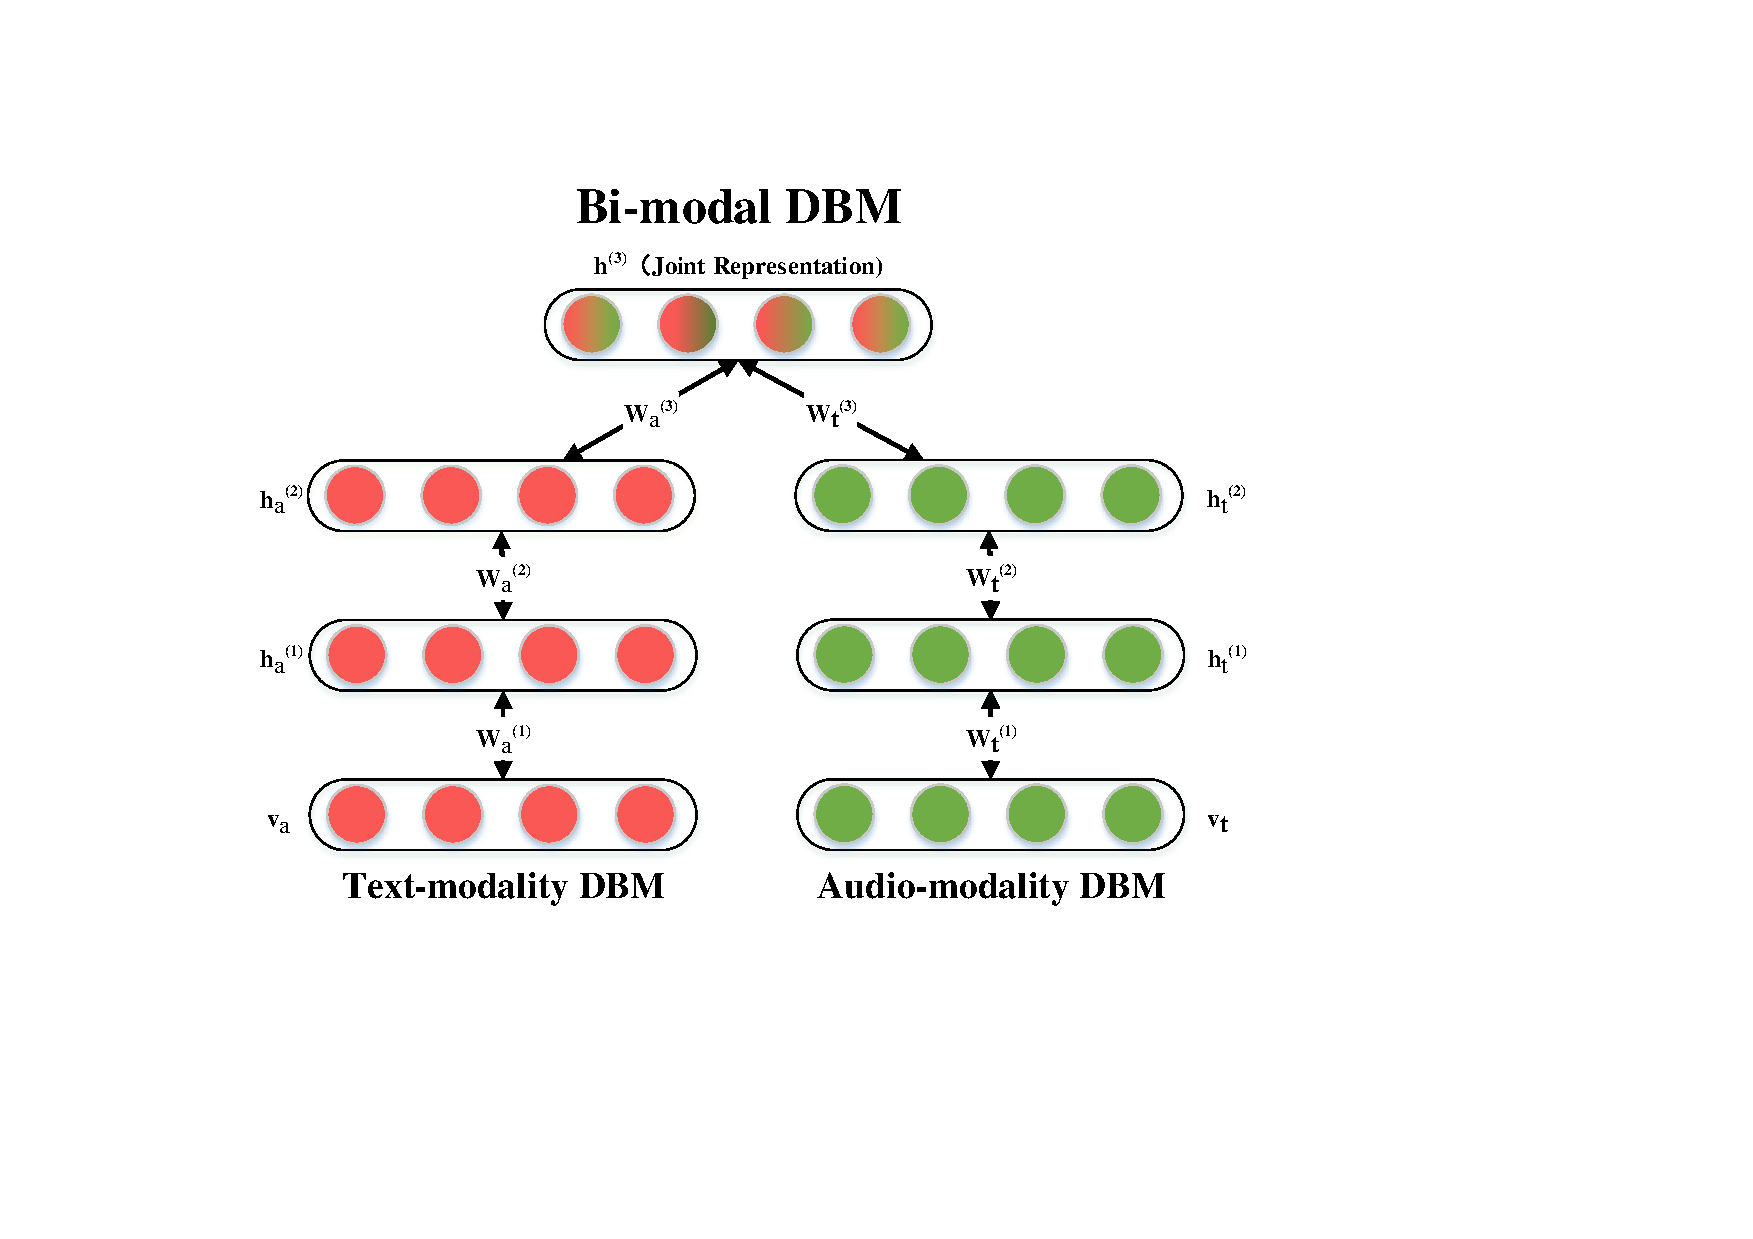
\includegraphics[width=0.5\columnwidth]{figures/bi-modalDBM}
	%  \setlength{\abovecaptionskip}{0pt}
	%  \setlength{\belowcaptionskip}{-20pt}
	\caption{Bi-modal Deep Boltzmann Machine}
	\label{fg:DBM}
\end{figure}

%We here mainly utilize second and third features of the multimodal DBM.
Multimodal DBM is a generative model for that can create fused representations by combining features from different modalities in a model fusion scheme~\cite{DBLP:journals/jmlr/SrivastavaS14}. %There are 3 main usages of multi-modal DBM: 1) Generating missing modalities; 2) Inferring joint representations; and 3) Discriminative tasks. After a greedy layer-wise pretraining stage \cite{DBLP:journals/jmlr/SalakhutdinovH09}, variational inference are used to approximate posterior $Q(\mathbf{h}^{(3)}|\mathbf{v}_{a}, \mathbf{v}_{t})$ and to obtain the joint representation of the multi-modal inputs. Softmax classifiers and Support Vector machine can then be trained with these fine-grained representations to do mood classifications. Note that 1) can also be exploited in the pre-training stage of our model, which makes the it an ideal model for classification in music moods.
Fig. \ref{fg:DBM} illustrates the proposed audio-text aware bi-modal DBM architecture; it consists of two 2-layer DBM networks, with an additional layer of hidden units added on top to join the two DBMs and form a single model. 

Let $\mathbf{v}_{a}\in\mathbb{R}^{D}$ denote the audio input and $\mathbf{v}_{t}\in\mathbb{R}^{K}$ denote the text input, where $K,D\in\mathbb{R}$ is the dimension of audio and text features. Then, the joint distribution of bi-modal input can be then written as:
\begin{equation}\label{eq3}
\begin{split}
P(\mathbf{v}_{a},\mathbf{v}_{t};\theta)=\sum_{\mathbf{h}_{\mathbf{a}}^{(2)},\mathbf{h}_{\mathbf{t}}^{(2)},\mathbf{h}^{(3)}} &P(\mathbf{h}_{\mathbf{a}}^{(2)},\mathbf{h}_{\mathbf{t}}^{(2)},\mathbf{h}^{(3)})\left(\sum_{\mathbf{h}_{\mathbf{a}}^{(1)}}P(\mathbf{v}_{a},\mathbf{h}_{\mathbf{a}}^{(1)}\mid \mathbf{h}_{\mathbf{a}}^{(2)})\right) \\
& \left(\sum_{\mathbf{h}_{\mathbf{t}}^{(1)}}P(\mathbf{v}_{t},\mathbf{h}_{\mathbf{t}}^{(1)}\mid \mathbf{h}_{\mathbf{t}}^{(2)})\right)
\end{split}
\end{equation}

The second term in~Eq. \ref{eq3} denotes the probability distribution of the audio modality, which assigns probability to $\mathbf{v}_{a}$ in a Gaussian RBM scheme:
\begin{equation}
\begin{split}\label{al1}
P(\mathbf{v}_{\mathbf{a}};\theta_{a}) &= \sum_{\mathbf{h}_{\mathbf{a}}^{(1)},\mathbf{h}_{\mathbf{a}}^{(2)}}P(\mathbf{v}_{\mathbf{a}},\mathbf{h}_{\mathbf{a}}^{(2)},\mathbf{h}_{\mathbf{a}}^{(1)};\theta_{a}) \\
&= \frac{1}{\mathit{Z}(\theta_{a})}\sum_{\mathbf{h}_{\mathbf{a}}^{(1)},\mathbf{h}_{\mathbf{a}}^{(2)}}exp\left(-\sum_{i}\frac{{(v_{\mathbf{a}i}-b_{\mathbf{a}i})}^{2}}{2\sigma_{i}^{2}}+\sum_{ij}\frac{v_{\mathbf{a}i}}{\sigma_{i}}W_{\mathbf{a}ij}^{(1)}h_{\mathbf{a}j}^{(1)}+\right. \\
&\left.\qquad\sum_{jl}W_{\mathbf{a}jl}^{(1)}h_{\mathbf{a}j}^{(1)}h_{\mathbf{a}l}^{(2)}+\sum_{j}b_{\mathbf{a}j}^{(1)}h_{\mathbf{a}j}^{(1)}+\sum_{l}b_{\mathbf{a}l}^{(2)}h_{\mathbf{a}l}^{(2)}\right)
\end{split}
\end{equation}

The third term in~Eq. \ref{eq3} denotes the probability distribution of the text modality, where $\mathbf{v\in \mathbb{N}^{k}}$ denotes a vector of visible units and each ${v}_{k}$ is the number of times word $k$ occurs in the lyrics with the dictionary size $M$. The model assigns probability to $\mathbf{v}_{t}$ in a Replicated Softmax RBM scheme:
\begin{equation}
\begin{split}\label{al2}
P(\mathbf{v}_{\mathbf{t}};\theta_{t}) &= \sum_{\mathbf{h}_{\mathbf{t}}^{(1)},\mathbf{h}_{\mathbf{t}}^{(2)}}P(\mathbf{v}_{\mathbf{t}},\mathbf{h}_{\mathbf{t}}^{(2)},\mathbf{h}_{\mathbf{t}}^{(1)};\theta_{t}) \\
&= \frac{1}{\mathit{Z}_{M}(\theta_{t})}\sum_{\mathbf{h}_{\mathbf{t}}^{(1)},\mathbf{h}_{\mathbf{t}}^{(2)}}exp\left(\sum_{jk}W_{\mathbf{t}k,j}^{(1)}h_{\mathbf{t}j}^{(1)}v_{\mathbf{t}k}+\sum_{jl}W_{\mathbf{t}jl}^{(2)}h_{\mathbf{t}j}^{(1)}h_{\mathbf{t}l}^{(2)}+\right. \\
&\left.\qquad\sum_{k}b_{\mathbf{t}k}v_{\mathbf{t}k}+M\sum_{j}b_{\mathbf{t}j}^{(1)}h_{\mathbf{t}j}^{(1)}+\sum_{l}b_{\mathbf{t}l}^{(2)}h_{\mathbf{t}l}^{(2)}\right)
\end{split}
\end{equation}

The parameters of DBM can be initialised randomly. However, here we use a greedy layer-wise pre-training strategy~\cite{DBLP:journals/jmlr/SalakhutdinovH09,DBLP:journals/jmlr/SrivastavaS14}. %by learning a stack of modified Restricted Boltzmann Machines, which enables the DBM to perform much better~\cite{DBLP:journals/jmlr/SalakhutdinovH09,DBLP:journals/jmlr/SrivastavaS14}.

\section{Experimental Study}
%\subsection{Dataset Configuration}
%along with rich music metadata.
In our experiments, we use 
% perform the experiment on a dataset derived from MusixMatch%\footnote[1]{https://www.musixmatch.com/}, a subset of
the largest publicly available music dataset, the Million Song Dataset (MSD)~\cite{DBLP:conf/ismir/Bertin-MahieuxEWL11}. %which consists of approximately 1,000,000 music tracks. 
It is a conglomeration of several datasets containing different information about the tracks; we use two of its subsets. First, MusiXmatch, contains information about the lyrics,	  %Rich audio-derived features such as Mel Frequency Cepstral Coefficients (MFCC), Statistical Spectrum Descriptors (SSD) and Rhythm Patterns (RP) are found in the MSD Benchmarks. %\footnote[1]{http://www.ifs.tuwien.ac.at/mir/msd/}.
each song is described as a set of words from the recorded top 5,000 frequent words across all lyrics. Second, Last.fm, contains annotations obtained from music listeners in a form of tags, like ``happy'' and ``upbeat''; from it, we select tracks that are described by emotion related tags. Additionally, we obtain already pre-extracted audio-based features from the MSD Benchmarking dataset, which is an extension of MSD and was created for the purposes of comparing different approaches while maintaining invariability in various experimental parameters~\cite{schindler1}. To capture both modalities, in our experiments, each music track is represented by both lyrics (found in MusiXmatch dataset) and audio-based features (from MSDB dataset), there are 236,486 tracks that satisfy these conditions. 


Initially, to test the validity of our approach, we select only the tracks that contain ``happy'' and ``sad'' tags. After removing ambiguous tracks that contain both tags, we obtain 7,945 ``happy'' songs and 5,840 ``sad'' tracks. To avoid classifier bias due to class imbalance, we perform random subsampling and then conduct a binary emotion classification experiment. %(described later in this section).

% both audio features and lyrics are selected to constitute the dataset. In text modality, each song is described as a set of words from the recorded top 5,000 frequent words across all lyrics. Afterwards, Last.fm\footnote[2]{http://www.last.fm/} is used to extract emotional tags for the songs in the dataset. However,
In a multi-class scenario, some songs may cover a variety of emotions, rendering the representation by independent dimensions inadequate. For this reason, we employ Russell's Valence-Arousal model~\cite{Russell1980} and follow Corona's and O'Mahony's scheme of selecting social tags that clearly indicate the song's emotional trend~\cite{Corona2015An}. %We find that some tags describe no more than a hundred songs and are not suitable for training a classifier, we then merged such tags into one single group,
We group the tags according to their quadrants in the Valence-Arousal model and report the final number of tracks tagged by each emotion group in Table \ref{tb:clas-scheme}. We use the tracks that have the emotion-related tags as labelled data for training the classifier, and the remainder as unlabelled data for unsupervised pre-training. % stage described in Section 3. 
Our final dataset contains 41,727 labelled and 194,759 unlabelled tracks.%, with labeled data account for 17.6\% of the whole data.

%Among the 237,663 songs from MusixMatch, 236,486 songs which contains both audio features and lyrics are selected to constitute the dataset. In text modality, each song is described as a set of words from the recorded top 5,000 frequent words across all lyrics. Afterwards, Last.fm\footnote[2]{http://www.last.fm/} is used to extract emotional tags for the songs in the dataset. However, some songs may cover a variety of emotion. Independent dimensions are thus inadequate to represent the classification task. Here we employ Russell's Valence-Arousal model \cite{Russell1980} and follow the classifying scheme in \cite{Corona2015An} to select social tags that clearly indicates the song's emotional trend. It is found that some selected tags only contain no more than 100 songs and are not suitable for training a classifier, we then merged such tags into one single group, according to their quadrants in the Valence-Arousal model. The final number of songs tagged by each emotion group is shown in Table \ref{tb:clas-scheme}. Songs that have the emotional tags are labeled data for training the classifiers, while the rest of them are unlabeled data for the pretraining stage described in Section 3. The resulting dataset contains 41,727 labeled songs and 194,759 unlabeled songs, with labeled data account for 17.6\% of the whole data.

%while lyric features are from MusixMatch dataset, which has 237,663 songs with lyric modality information and describes each song by a set of words from the recorded top 5,000 frequent words across all lyrics. %As there exist many copyright issues towards music lyrics, and this work mainly focus on proposing a proper model for classification, so we using the readily available basic level lyric features, e.g. bag-of-words(BOW) of every song. Examples of the BOW feature of songs are shown in \ref{table1}.

%\begin{table}[]
%	\centering
%	\begin{tabular}{|l|l|}
%		\hline
%		\multicolumn{1}{|c|}{\textbf{emotion tags}} & \multicolumn{1}{c|}{\textbf{appeared words}}                                                                                                                                          \\ \hline
%		aggressive,regret                           & \begin{tabular}[c]{@{}l@{}}wrong, blood, place, face, scare, gun, fear, dead, real, pain, time,\\ head, cause, your.\end{tabular}                                                      \\ \hline
%		sad,blue                                    & \begin{tabular}[c]{@{}l@{}}her, heartbreak, fairy, tale, white, sacrifice, stood, page, gold, saw,\\ line, hard, wait,letter, light, turn, still, warm, write, bone, sea.\end{tabular} \\ \hline
%	\end{tabular}
%	\caption{Examples of BOW lyric features. The appeared words are top words after weighted by tf-idf. We also did un-stem of these words to better illustrate the relations between emotions and lyrics.}
%	\label{table1}
%\end{table}

%which is tagged by online users. Among the super noisy tags, there is a subset that clearly indicates the emotion of the tagged song.

%For example, Bohemian Rhapsody by Queen is comprised of moods like angry, sadness, regret, etc.

%Last.fm\footnote[1]{http://www.last.fm/} is used in this research to extract emotional tags of a song in the MusixMatch dataset. However, music emotion classification is difficult due to people's different culture \cite{Song2013Do} and perception \cite{Kosta2013A}. Some songs may cover a variety of emotion. Independent dimensions are thus inadequate to represent the classification task. Here we employ Russell's Valence-Arousal model \cite{Russell1980} and follow the classifying scheme in \cite{Corona2015An} to select social tags that clearly indicates the song's emotional trend. It is found that some selected tags only contains no more than 100 songs and is not suitable for training a classifier, we then merged such tags into one single group, according to their quadrants in the Valence-Arousal model. The final number of songs tagged by each emotion group is shown in Table \ref{tb:clas-scheme}.


%Russell's Valence-Arousal model maps every mood into a 2-dimensional space defined by valence (good–bad dimension of sentiment) and arousal (active–passive dimension of sentiment). It is one of the most widely used ontology for classifying moods and is thus adopted in our classification task. Follow the classifying scheme in \cite{Corona2015An}, we select some social tags from last.fm that clearly indicates the song's emotional trend. As some selected tags only contains no more than 100 songs and is not suitable for training a classifier, we then merged several tags into one single group, according to their quadrants in the Valence-Arousal model. The final number of songs tagged by each emotion group is shown in \ref{tb:clas-scheme}. It can be seen that even after the merge, some quadrants still have a relatively small number of songs, e.g. $v^{+}a^{-}$ quadrant.

\begin{table}
	\centering
	\caption{Mood quadrants and their corresponding number of songs}
	\label{tb:clas-scheme}
	\begin{tabular}{|c|l|l|c|}
		\hline
		\textbf{Quadrant}               & \multicolumn{1}{c|}{\textbf{Group}} & \multicolumn{1}{c|}{\textbf{Tag}} & \textbf{Songs}         \\ \hline
		\multirow{2}{*}{$v^{-}a^{+}$} & G29                                 & aggressive,aggression.            & \multirow{2}{*}{28,168} \\ \cline{2-3}
		& G28                                 & anger,angry,choleric,etc.         &                         \\ \hline
		\multirow{2}{*}{$v^{+}a^{+}$} & G6                                  & cheerful,jolly,festive,etc.       & \multirow{2}{*}{16,315} \\ \cline{2-3}
		& G5                                  & happy,happiness,etc.              &                         \\ \hline
		\multirow{3}{*}{$v^{-}a^{-}$} & G15                                 & sad,sadness,unhappy,etc.          & \multirow{3}{*}{10,154} \\ \cline{2-3}
		& G16                                 & depressed,blue,dark,gloom,etc.    &                         \\ \cline{2-3}
		& G17                                 & heartbreak,grief,sorrow,etc.      &                         \\ \hline
		\multirow{2}{*}{$v^{+}a^{-}$}  & G8                                  & brooding,contemplative,etc.       & \multirow{2}{*}{2,629}  \\ \cline{2-3}
		& G12                                 & calm,comfort,quiet,etc.           &                         \\ \hline
	\end{tabular}
\end{table}

%As a result, we select totally 236,486 songs that does contain lyric information. According to \ref{tb:clas-scheme}, songs that have the emotional tags are selected as labeled data for training the classifiers, while the rest of them are unlabeled data for the pretraining stage described in Section 3. The resulting dataset contains 41,727 labeled songs and 194,759 unlabeled songs, with labeled data account for 17.6\% of the whole data.

%\subsection{Valence-Arousal model}
%People's different culture \cite{Song2013Do} and perception \cite{Kosta2013A} makes music moods difficult to classify. Some songs may also cover a variety of moods. For example, Bohemian Rhapsody by Queen is comprised of moods like angry, sadness, regret, etc. Independent dimensions are thus inadequate to represent the classification task. Russell’s model of affection maps every mood into a 2-dimensional space defined by valence(good–bad dimension of sentiment) and arousal(active–passive dimension of sentiment). It is one of the most widely used ontology for classifying moods. Besides, since more complicated classification approaches seem redundant towards our task, we adopted the Valence-Arousal model in our classification task. Follow the classifying scheme in \cite{Corona2015An}, we group the moods into 4 main categories according to the 4 quadrants of Russell’s model in order to build a big and representative dataset.

%\begin{figure}
%  \centering
%  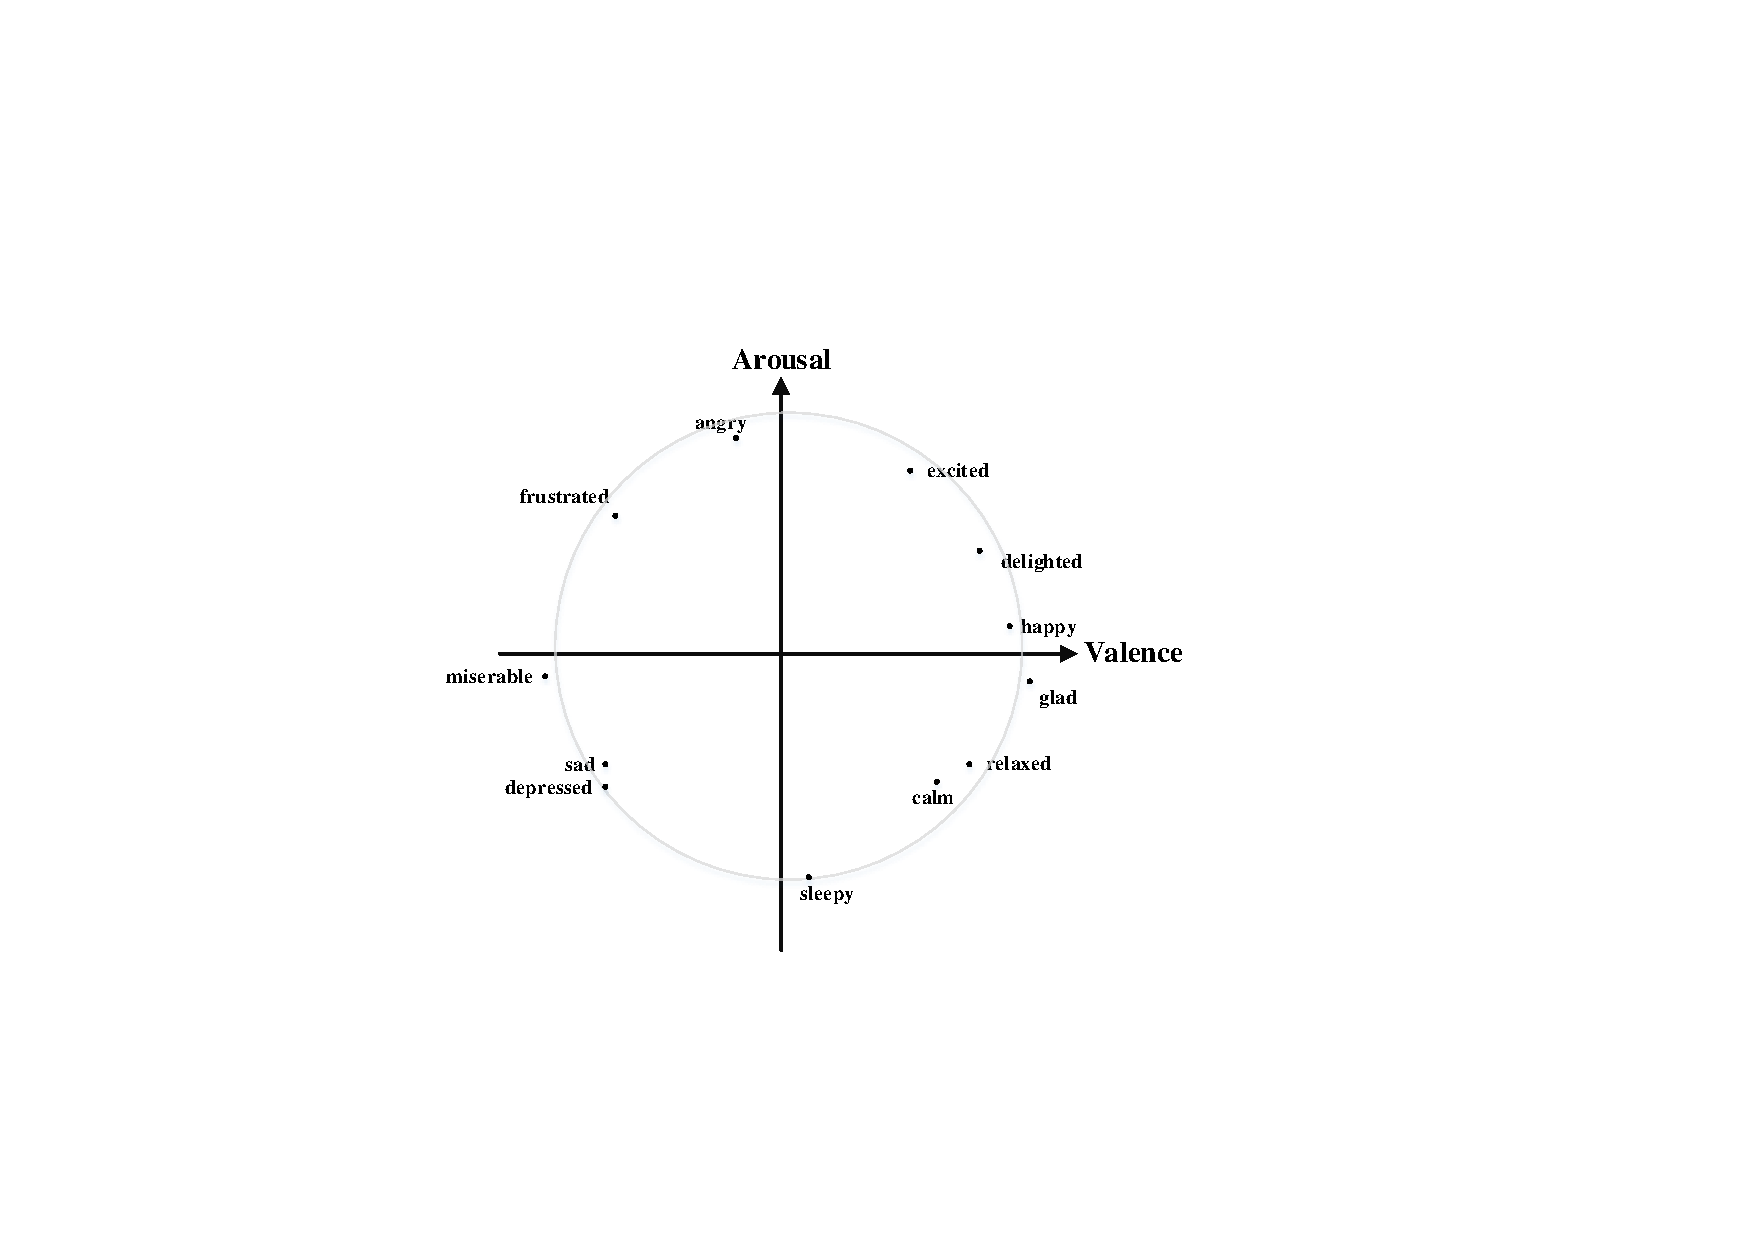
\includegraphics[width=0.5\columnwidth]{figures/v-a_model}
%  \setlength{\abovecaptionskip}{0pt}
%  \setlength{\belowcaptionskip}{-20pt}
%  \caption{Bi-modal Deep Boltzmann Machine}\label{fg:va-Model}
%\end{figure}

%\subsection{Binary Emotion Classification}

%In this experiment we mainly focus on the bi-modal DBM’s ability to fuse the two information modality. Hence, we only did a binary mood classification between happy and sad. As happy and sad are totally opposing emotions. Nevertheless, there is still 720 songs that are both tagged with happy and sad. We thus removed these songs to avoid ambiguity. 7,945 Songs are tagged with 'happy' while 5,840 songs are tagged with 'sad'. To ensure the two mood class is equally treated, we randomly pick 5,840 'happy' songs to comprise a 11,680 songs dataset with 1:1 sample ratio.



The deep learning architecture is configured as following. The audio pathway is modeled by an  RBM with 194 visible units, each taking as input acoustic content descriptors, such as MFCC and SSD features. The visible layer is followed by two layers of hidden units, 100 and 50 each. The text modality is formed by RBM consisting of 5,000-unit visible layer followed by hidden layers of 2,048 and 1,024 units each. A joint layer combines the two modalities and consists of 1,074 hidden units. Its output can be considered as a complex probability estimate of the mood classes. We use the output from our Mulimodal RBM as input to either Softmax or SVM for the final classification decision. Additionally, to test the robustness of our chosen audio features, we expand the audio modality from 194 to 3,456 dimensions by including additional audio-based features. The hidden layers are also expanded to 2,048 and 1,024 respectively; and the joint layer to 2,048 units.


%Furthermore, to see how feature selection strategy influence the classification accuracy, we expand the feature on audio modality to 3456 dimensions by including features such as rhythm patterns, Temporal statistical spectrum descriptors, etc. Hidden units in the hidden layer are also expanded to 2,048-1,024, and the joint layer now contains 2,048 hidden units. 

%Parameters were pretrained using PCD for initialisation, and all word counts vectors are scaled to 5 to avoid running separate Markov Chains for each word counts to get the model distribution's sufficient statistics \cite{DBLP:journals/jmlr/SrivastavaS14}.
%For the classification, both SVM and Softmax are used on each layer of representation. 
%Here we only report the result using SVM, as it is slightly better. 
Because the SVM classifier performs slightly better on average, we omit the Softmax results. In our experiments, we perform $k$-fold repeated random sub-sampling validation with $k=5$. In each fold, 60\% (6,984) tracks are selected for training and 40\% (4,656) for testing. We compute Mean Average Precision (MAP) %, Prec@n 
and Accuracy as metrics to comprehensively evaluate the models. %We arbitarily set n to 50 according to \cite{DBLP:conf/sigir/BuckleyV00}. 
The initial experimental results are shown in Fig. 2, %To show the performance, Mean Average Precision (MAP), Prec@50 and Accuracy is used as metrics to comprehensively evaluate the models. The experimental results are shown in Fig. 2.
where we also illustrated the baseline SVM performance (no DBM) using early concatenation method to join the two modalities into a single input vector.


\begin{figure}
	\centering
	\label{fg:performance}
	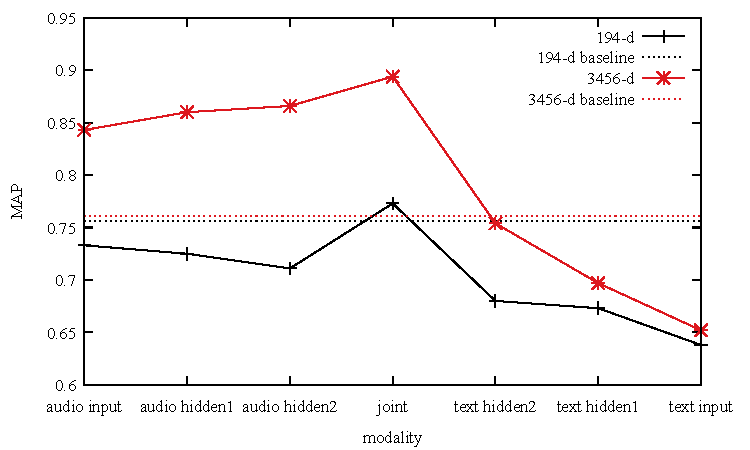
\includegraphics[width=.495\textwidth]{figures/map}
	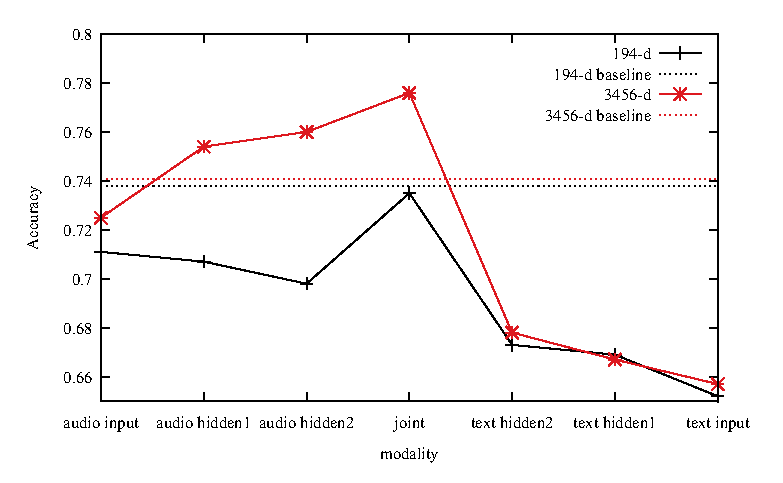
\includegraphics[width=.495\textwidth]{figures/acc}
%	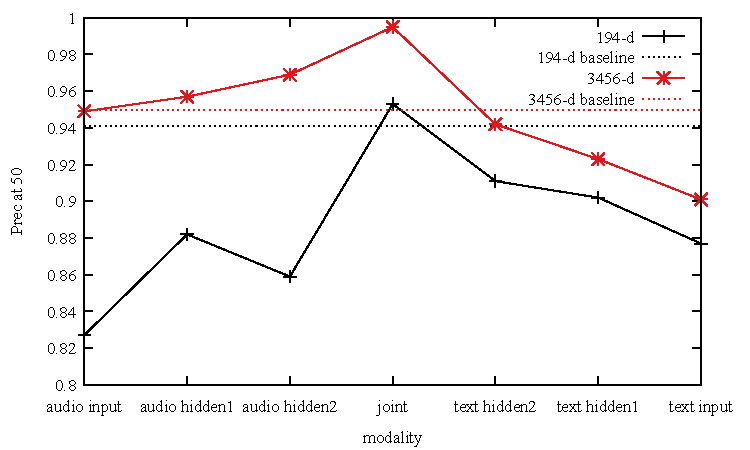
\includegraphics[width=.3\textwidth]{figures/prec@50}
	\caption{MAP and Accuracy achieved by the Bi-modal Boltzmann Machine in the ``happy''/``sad'' binary classification task}%and Prec@50 achieved by the Bi-modal Boltzmann Machine.}
\end{figure}

%\subsection{Discussion}
%\subsubsection{Fusing Ability}
As can be seen from Fig. 2, audio-based features indeed outperform the lyric-based features to some extent. We conjecture that this may be because the audio modality is represented by features that were hand-crafted and improved over the years. Meanwhile, the text modality is represented by a shallow BoW statistical measure with large vocabulary, which results in a sparse input vector. This again urges the study on higher level lyric features, which may yield interesting results. 
We also noticed that the classification performance declined through the audio pathway, which indicates that some valuable information are lost through the extracting process in the audio modality. 
%This it is caused by the insufficient number of audio features. 
After expanding the audio modality with additional features, this phenomenon disappears. This indicates the necessity of feature selection. %, for both deficiency and redundancy of features may all cause poor performance.
Among all results, the best performance is achieved at the joint layer, which shows the effectiveness of the fusing ability of the proposed approach. After expanding the audio features from 194 to 3,456, the baseline SVM performance did not improve much. %since simple concatenation yields an 8456-dimension feature vector that is hard to find a decision boundary. However, our model can easily handle high dimensionality classification problem by gradually mapping it into lower-dimension vector spaces. 



%\subsection{Multi-emotion Classification}
%As music may be labeled by several different tags, did 1-vs-all classification using SVM on the input and top joint layer for each mod group respectively.
%After testing the binary emotion task classification, we further evaluate the model's performance on multi-mood classification tasks. Besides 
In addition to using the lyric- and audio-based features with our approach, we also compare the model fusion, early fusion and late fusion methods. In late fusion, we first trained two SVM classifiers to represent the two modalities separately, denoting as $p_{a}$ and $p_{t}$. Then the output mood class is assigned by
\begin{equation}
p = \alpha p_{a}+(1-\alpha)p_{t}
\end{equation}
where $\alpha$ indicates the relevant importance between audio and lyric features. We set $\alpha = 0.6$, as per Hu et al.~\cite{Hu2016A}. As before, in order to avoid classifier bias towards majority class, we attempt to maintain class balance by ensuring that both training and testing instances are equally distributed across mood classes. 
%Similar to binary emotion classification, we randomly constructed the training and testing set with 40\% positive samples and 60\% negative samples. The negative samples are equally distributed across three negative mood classes, in order to ensure the classifier to get familiar with each type of negative samples. 
Results are shown in Table \ref{tb:multimood-rst}.


\begin{table}[!hpt]
	\centering
	\caption{Comparison of accuracy achieved by the different fusion models}
	\label{tb:multimood-rst}
	\begin{tabular}{|c|c|c|c|c|c|}
		\hline
		& \textbf{audio\_only} & \textbf{text\_only} & \textbf{early\_fusion} & \textbf{late\_fusion} & \textbf{Bi-modal DBM} \\ \hline
		$v^{-}a^{+}$ & 0.645               & 0.600                & 0.689                 & 0.666                & \textbf{0.706}                 \\ \hline
		$v^{+}a^{+}$ & 0.625               & 0.607              & 0.653                 & 0.639                & \textbf{0.692}                 \\ \hline
		$v^{-}a^{-}$ & 0.634               & 0.620               & 0.661                 & 0.642                & \textbf{0.704}                 \\ \hline
		$v^{+}a^{-}$ & 0.730               & 0.702              & 0.745                 & 0.729                & \textbf{0.785}                 \\ \hline
	\end{tabular}
\end{table}

%\subsection{Discussion}
%\subsubsection{Fusing Ability}
Our model outperformed other baseline models in every mood category. The moods in $v^{+}a^{-}$ quadrant obtain the highest accuracy. This is interesting given that the $v^{+}a^{-}$ quadrant has the least number of songs. The reason may be that music pieces in this mood group has many unique lyric terms. Between other mood categories, however, there is no significant differences in the classification accuracy. Moreover, the fusion methods' accuracy all outperformed the accuracy of classification on single modality, affirming the effectiveness of multi-modal mood classification in the same way as many prior studies show.


\section{Conclusion}% and Future Works}
In this work, we used a deep learning architecture, inspired by the work of Srivastava and Salakhutdinov~\cite{DBLP:journals/jmlr/SrivastavaS14}, to effectively fuse the audio and text modalities for music mood classification. 
Results show that fusing modalities is indeed advantageous in the music mood classification task. In addition to including information from other domains/modalities, it would be interesting to see how other lyric derived features perform with this and other multimodal approaches in the music-IR literature, we leave this to our future work.
%Results show that the bi-modal DBM outperforms than single modality and other multi-modal baseline models across every emotion group. It also showed flexibility towards high dimensional inputs. It is expected that this work can provide insight for future research in this direction.%Besides, we also built a large dataset basing on the Million Song Dataset. As urged by \cite{Corona2015An} and \cite{Hu2016A}, we plan to make our dataset available and add higher level lyric features for deeper analysis by integrating semantic information.

\subsubsection*{Acknowledgements}
This work was partially supported by the National Natural Science Foundation of China (No. 61332018), the National Department Public Benefit Research Foundation (No. 201510209), and the Fundamental Research Funds for the Central Universities.

\bibliographystyle{splncs03}
%\bibliographystyle{unsrt}
\bibliography{reference}
	
\end{document}
